\documentclass[a4paper,11pt]{article}
\usepackage{booktabs}   % for professional table rules
\usepackage{caption}    % for customizing captions
\usepackage{array}      % for better column formatting
\usepackage{siunitx}    % for consistent units
\usepackage{graphicx}   % for importing figures
\usepackage{geometry}   % for page margins
\usepackage{amsmath}    % for math alignment
\usepackage{amssymb}    % for math symbols
\usepackage{float}      % for [H] figure placement
\usepackage{hyperref}   % for links and references
\usepackage{multirow}   % for multirow in tables
\usepackage{fouriernc}
\geometry{left=2cm,right=2cm,top=2cm,bottom=2.5cm}
\hypersetup{
    colorlinks=true,
    linkcolor=blue,
    filecolor=magenta,      
    urlcolor=cyan,
    pdftitle={Lab Report: The Photoelectric Effect},
    pdfpagemode=FullScreen,
}

\begin{document}

% ------------------- Title / Cover Page -------------------
\noindent
\begin{center}
    
\includegraphics[width=0.25\textwidth]{sut.jpg} \\
    \vspace{2pt}
\end{center}
\begin{center}
    {\LARGE \bf Department of Physics} \\
    \vspace{2pt}
    {\Large \bf Sharif University of Technology} \\
    \vspace{8pt}
    {\large \bf Physics Lab IV --- General Physics Laboratory} \\
    \vspace{4pt}
    \hrule
    \vspace{6pt}
    {\Large \bf Experiment Report: The Photoelectric Effect}
\end{center}
\hrule
\vspace{0.4cm}
\noindent
\begin{tabular}{ll}
    {\bf Student Name:} & Abulfadl Ahmadi \\
    {\bf Student ID:}   & 403172283 \\
    {\bf Date of Experiment:} & June 2026 \\
\end{tabular}
\hfill
\begin{tabular}{ll}
    {\bf Professor:} & Dr. Khademi \\
    {\bf Teaching Assistants:} & Yasin Amiri \\
    & Sonia \\
\end{tabular}

\vspace{0.6cm}

% ------------------- Abstract -------------------
\begin{abstract}
This experiment investigates the photoelectric effect to confirm the quantum nature of light and determine Planck's constant ($h$) alongside the work function ($\Phi$) of a photocathode material. By irradiating a photocell with monochromatic light from a high-pressure mercury lamp, the resulting photocurrent is measured as a function of an applied retarding voltage. The stopping potentials ($U_0$) are meticulously recorded across five different optical frequencies ranging from $5.19 \times 10^{14}\text{ Hz}$ to $7.41 \times 10^{14}\text{ Hz}$. An Ordinary Least Squares (OLS) linear regression of $U_0$ against frequency $\nu$ yields an experimental value for Planck's constant of $h = (2.26 \pm 0.69) \times 10^{-34}\text{ J}\cdot\text{s}$ and a work function of $\Phi = -0.085 \pm 0.268\text{ eV}$. While the fundamental linear relationship predicted by Einstein's photoelectric equation is observed, the steep relative error ($65.8\%$) emphasizes the presence of significant systematic anomalies, primarily uncompensated contact potentials, dark currents, and reverse photoemission, which drastically dampen the experimental slope.
\end{abstract}

% ------------------- Section 1: Objectives -------------------
\section{Objectives}
The primary objectives of this experiment are:
\begin{enumerate}
    \item To observe the photoelectric effect and plot the photocurrent-voltage ($I-V$) characteristic curves for different frequencies of incident light.
    \item To measure the stopping potential ($U_0$) required to halt the emission of photoelectrons for various spectral lines of a mercury lamp.
    \item To utilize Ordinary Least Squares (OLS) regression on the $U_0$ vs. $\nu$ data to experimentally determine Planck's constant ($h$) and the work function ($\Phi$).
    \item To analyze the limitations of classical physics in explaining this phenomenon and discuss the systemic sources of error inherent in the experimental setup.
\end{enumerate}

% ------------------- Section 2: Theoretical Background -------------------
\section{Theoretical Background}
When electromagnetic radiation illuminates a metallic surface, electrons can be ejected from the material. This phenomenon, known as the photoelectric effect, cannot be adequately explained by the classical wave theory of light. Classical physics incorrectly predicts that the kinetic energy of emitted electrons should depend on the light's intensity and that emission should occur at any frequency given sufficient time to accumulate energy.

In 1905, Albert Einstein resolved this by proposing that light consists of discrete energy quanta, later called photons. The energy of a single photon is strictly proportional to its frequency $\nu$:
\begin{equation}
    E = h \nu
\end{equation}
where $h$ is Planck's constant. For an electron to be freed from the atomic lattice, the incoming photon must possess an energy greater than or equal to the material's work function ($\Phi$), which is the minimum binding energy of an electron at the surface. 

By conservation of energy, the maximum kinetic energy ($K_{\text{max}}$) of the ejected photoelectron is the energy of the absorbed photon minus the work function:
\begin{equation}
    K_{\text{max}} = \frac{1}{2} m v_{\text{max}}^2 = h \nu - \Phi
\end{equation}
Experimentally, this kinetic energy can be measured by applying a negative retarding (or stopping) potential $U_0$ across the anode and cathode. The minimum voltage required to completely halt the photocurrent $I$ satisfies the condition:
\begin{equation}
    e U_0 = K_{\text{max}} \implies e U_0 = h \nu - \Phi
\end{equation}
where $e$ is the elementary charge. Rearranging this equation yields a linear relationship between the stopping potential and the frequency of the incident light:
\begin{equation}
    U_0 = \left( \frac{h}{e} \right) \nu - \left( \frac{\Phi}{e} \right)
\end{equation}
By plotting $U_0$ against $\nu$, the slope of the line corresponds to $h/e$, and the y-intercept corresponds to $-\Phi/e$. This provides a direct empirical method for calculating Planck's constant.

% ------------------- Section 3: Experimental Setup & Uncertainties -------------------
\section{Experimental Setup \& Instrumental Uncertainties}
The experimental apparatus consists of a high-pressure mercury lamp as the photon source, optical filters to isolate specific spectral lines, and a photocell connected to an amplifier and a sensitive micro-ammeter. The photocell cathode is coated with a low-work-function material (typically an alkali metal like Potassium) to facilitate photoemission in the visible spectrum. The anode is shaped as a thin platinum ring to minimize the obstruction of incoming light.

For each selected color (Violet, Blue, Green-Blue, Green, Yellow), the monochromatic light strikes the cathode, generating a photocurrent. A variable DC voltage source applies a retarding potential until the ammeter registers exactly zero current. 

The assumed precision limits (instrumental errors) for the multimeters used in this configuration are:
\begin{itemize}
    \item Voltmeter uncertainty: $\delta U = 0.001\text{ V}$
    \item Ammeter uncertainty: $\delta I = 0.1\text{ A}$ (relative to the amplified scale display).
\end{itemize}

% ------------------- Section 4: Experimental Data \& Error Propagation -------------------
\section{Experimental Data, Regressions \& Error Propagation}

\subsection{Photocurrent vs. Retarding Voltage ($I-V$ Curves)}
The photocurrent $I$ was measured as a function of the applied retarding voltage $U$ for Violet and Green incident light. The data is presented in Table~\ref{tab:iv_data} and visually plotted in Figure~\ref{fig:iv_curve}.

\begin{table}[H]
\centering
\caption{Photocurrent $I$ as a function of the retarding potential $U$ for Violet and Green incident light.}
\label{tab:iv_data}
\begin{tabular}{l c c}
\toprule
Current $I$ (A) & Violet Voltage $U$ (V) & Green Voltage $U$ (V) \\
\midrule
$3.0$ & $0.737$ & $0.44$ \\
$2.8$ & $0.766$ & $0.45$ \\
$2.6$ & $0.750$ & $0.46$ \\
$2.4$ & $0.807$ & $0.47$ \\
$2.2$ & $0.833$ & $0.48$ \\
$2.0$ & $0.847$ & $0.49$ \\
$1.8$ & $0.871$ & $0.51$ \\
$1.6$ & $0.895$ & $0.52$ \\
$1.4$ & $0.921$ & $0.54$ \\
$1.2$ & $0.947$ & $0.55$ \\
$1.0$ & $0.976$ & $0.56$ \\
$0.8$ & $1.005$ & $0.58$ \\
$0.6$ & $1.048$ & $0.60$ \\
$0.4$ & $1.086$ & $0.64$ \\
$0.2$ & $1.147$ & $0.73$ \\
\bottomrule
\end{tabular}
\end{table}

\begin{figure}[H]
    \centering
    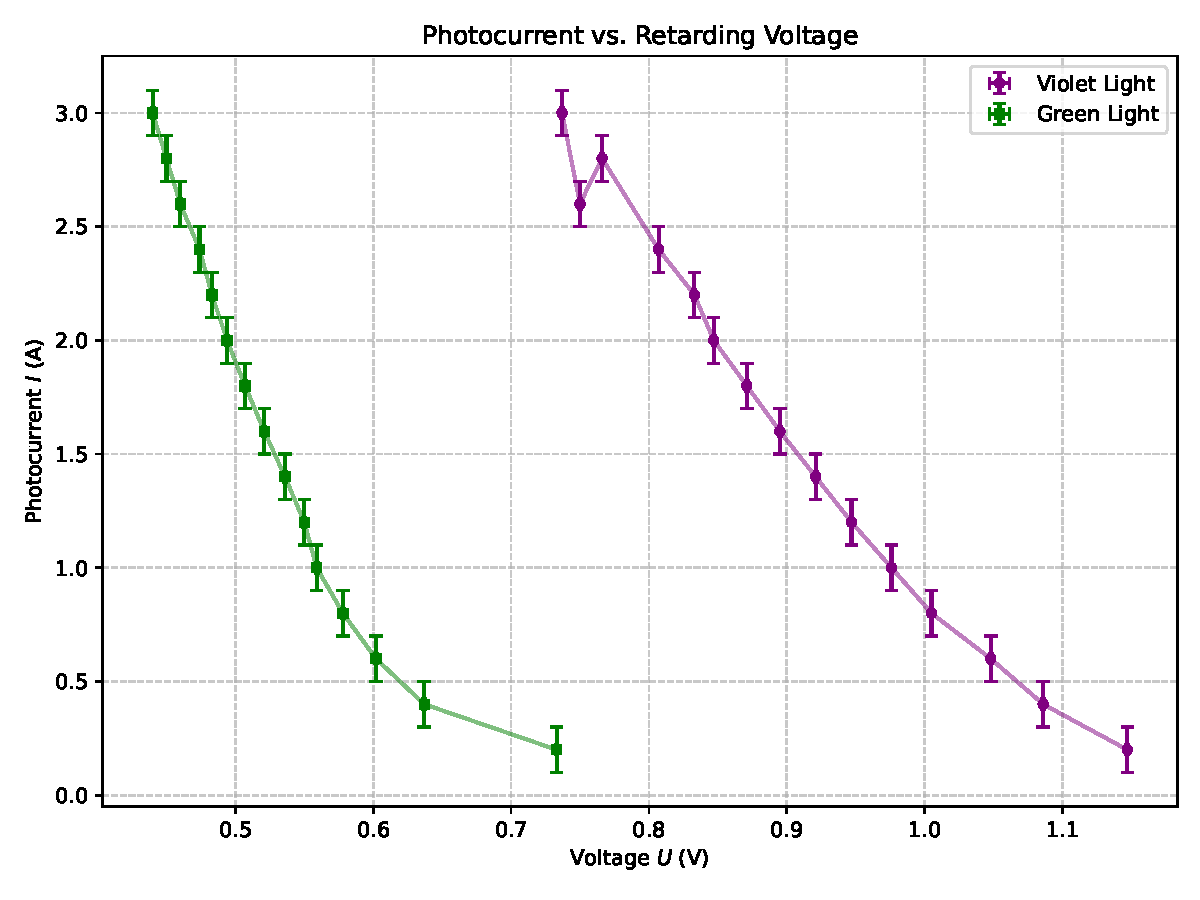
\includegraphics[width=0.8\textwidth]{plots/IV_curve.pdf}
    \caption{Photocurrent $I$ vs. Retarding Voltage $U$. The distinct x-intercepts highlight the frequency dependence of the stopping potential.}
    \label{fig:iv_curve}
\end{figure}

\subsection{Stopping Potential vs. Frequency \& OLS Regression}
To calculate Planck's constant, the exact stopping potential ($U_0$) was measured over three separate trials for five known frequencies of the mercury lamp. The standard error for $U_0$ at each frequency is defined as the maximum between the statistical standard error of the mean ($\sigma/\sqrt{3}$) and the instrumental tolerance ($\delta U$). The values are aggregated in Table~\ref{tab:u0_data}.

\begin{table}[H]
\centering
\caption{Measured stopping potentials ($U_0$) across three trials for different frequencies ($\nu$) of incident light.}
\label{tab:u0_data}
\begin{tabular}{lccccc}
\toprule
Frequency $\nu$ ($10^{14}$ Hz) & $5.19$ & $5.49$ & $6.10$ & $6.88$ & $7.41$ \\
Colour & Yellow & Green & Green-Blue & Blue & Violet \\
\midrule
$U_{0, \text{Trial 1}}$ (V) & 0.819 & 0.897 & 0.921 & 0.941 & 1.219 \\
$U_{0, \text{Trial 2}}$ (V) & 0.834 & 0.914 & 0.912 & 0.928 & 1.204 \\
$U_{0, \text{Trial 3}}$ (V) & 0.820 & 0.899 & 0.908 & 1.012 & 1.218 \\
\midrule
\textbf{Average $U_0$} (V) & $\mathbf{0.824 \pm 0.005}$ & $\mathbf{0.903 \pm 0.005}$ & $\mathbf{0.914 \pm 0.004}$ & $\mathbf{0.960 \pm 0.026}$ & $\mathbf{1.214 \pm 0.005}$ \\
\bottomrule
\end{tabular}
\end{table}

An Ordinary Least Squares (OLS) regression is performed on the average $U_0$ values against $\nu$ according to the model $y = m x + c$. 
The regression yields:
\begin{align*}
    \text{Slope (} h/e \text{)} &= (1.413 \pm 0.428) \times 10^{-15}\text{ V}\cdot\text{s} \\
    \text{Intercept (} -\Phi/e \text{)} &= 0.085 \pm 0.268\text{ V} \\
    R^2 &= 0.7843
\end{align*}

\begin{figure}[H]
    \centering
    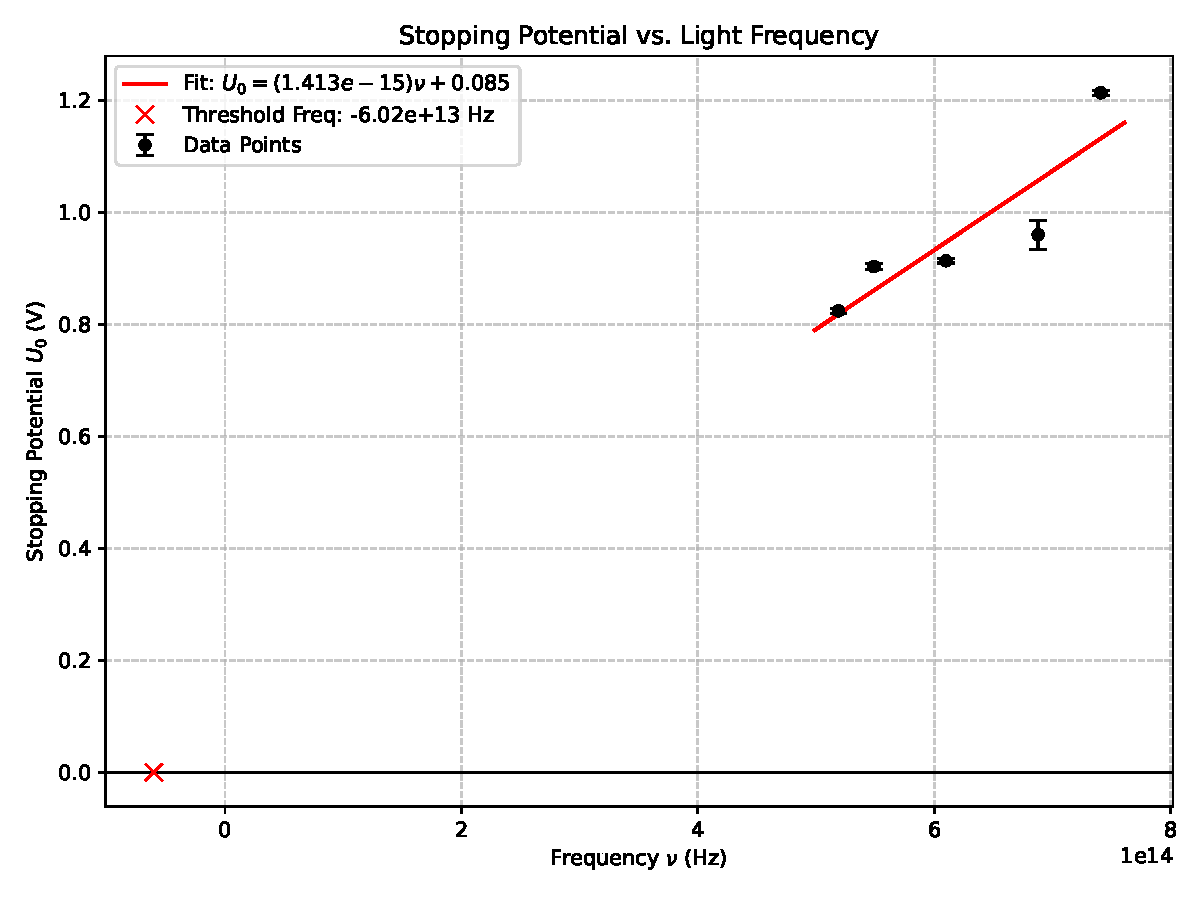
\includegraphics[width=0.8\textwidth]{plots/U0_vs_nu.pdf}
    \caption{Stopping Potential $U_0$ vs. Light Frequency $\nu$ with OLS regression line and error bars.}
    \label{fig:u0_vs_nu}
\end{figure}

By multiplying the slope and intercept by the elementary charge $e = 1.602 \times 10^{-19}\text{ C}$, we derive Planck's constant and the work function:
\begin{align*}
    h_{\text{exp}} &= (2.264 \pm 0.685) \times 10^{-34}\text{ J}\cdot\text{s} \\
    \Phi_{\text{exp}} &= -0.085 \pm 0.268\text{ eV}
\end{align*}
Comparing the experimental result to the accepted theoretical value of Planck's constant ($6.626 \times 10^{-34}\text{ J}\cdot\text{s}$), the relative error is $65.8\%$. This indicates a massive systematic underestimation of the slope, the physical causes of which are addressed in the post-lab questions.

% ------------------- Section 5: Post-Lab Questions -------------------
\section{Answers to Post-Lab Questions}

\subsection*{Q1: State the important physical result derived from this phenomenon.}
The most critical physical result is the confirmation of the \textbf{particle-like nature of light} and the quantization of electromagnetic energy. The experiment proves that light interacts with matter as discrete energy packets (photons) carrying exactly $E = h\nu$. Because the kinetic energy of the emitted electrons depends strictly on frequency and not on the wave intensity, classical wave mechanics is invalidated at the atomic scale, cementing the foundation of Quantum Mechanics.

\subsection*{Q2: Use the average stopping potentials to plot stopping potential vs. frequency. Determine Planck's constant and the work function from this curve.}
This request has been fulfilled in Section 4.2. As shown in Figure~\ref{fig:u0_vs_nu}, the OLS regression of the data points yields an experimental Planck's constant of $h = 2.26 \times 10^{-34}\text{ J}\cdot\text{s}$ and a mathematically extracted apparent work function of $\Phi = -0.085\text{ eV}$. (Note: A negative work function is physically impossible and reflects severe systematic errors shifting the intercept).

\subsection*{Q3: Given the theoretical value of Planck's constant, determine the relative percent error of the experiment and list the causes of error.}
The relative error is calculated as:
\begin{equation}
    \text{Error} = \frac{|2.264 - 6.626|}{6.626} \times 100 \approx 65.8\%
\end{equation}
This exceptionally high error stems from several systematic factors inherent to basic educational setups:
\begin{enumerate}
    \item \textbf{Contact Potential:} The cathode and anode are made of different metals with different work functions. This creates a built-in "contact potential" that shifts the measured stopping voltage indiscriminately.
    \item \textbf{Reverse Photoemission:} The anode, despite its ring shape, can reflect light or directly absorb scattered photons and emit electrons back toward the cathode, preventing the current from truly reaching a sharp zero point.
    \item \textbf{Thermionic Emission (Dark Current):} At room temperature, the low-work-function cathode emits a small number of electrons thermally, creating a background dark current that smears the $I-V$ intercept.
    \item \textbf{Filter Leakage:} Optical filters are imperfect and may allow a wide bandwidth of light to pass through. High-energy UV leakage can artificially inflate the stopping potential for lower frequency measurements.
\end{enumerate}

\subsection*{Q4: What is the work function and what factors does it depend on?}
The work function ($\Phi$) is the minimum thermodynamic work (energy) required to remove an electron from the solid bulk of a material to the vacuum immediately outside its surface. It heavily depends on:
\begin{itemize}
    \item \textbf{Chemical Composition:} The specific element and its atomic crystal lattice structure.
    \item \textbf{Surface Conditions:} The presence of impurities, oxidation layers, or specific coatings (e.g., alkali dopants) profoundly alters the surface dipole barrier, drastically changing $\Phi$.
\end{itemize}

\subsection*{Q5: Why is the velocity of the emitted electrons upon irradiation by monochromatic light not uniform?}
Electrons within a metal occupy a wide continuum of energy states up to the Fermi level. The work function $\Phi$ represents the energy required to liberate only the most loosely bound electrons (those exactly at the Fermi surface). Therefore, these specific electrons escape with the absolute maximum velocity ($v_{\text{max}}$). However, an incoming photon is equally likely to strike an electron sitting in a deeper energy band. Those deeper electrons require more energy to escape the lattice and subsequently emerge into the vacuum with much lower residual kinetic energy, resulting in a broad statistical distribution of velocities ranging from $0$ up to $v_{\text{max}}$.

\subsection*{Q6: State the cases that classical physics cannot explain in the photoelectric effect. How does modern physics answer them, and what cases can be explained by both?}
\textbf{Failures of Classical Physics:}
\begin{itemize}
    \item \textit{Kinetic Energy Dependence:} Classical waves suggest that higher light intensity (larger amplitude) should eject electrons with higher kinetic energy. Modern physics shows $K_{\text{max}}$ depends \textit{only} on frequency ($h\nu$).
    \item \textit{Threshold Frequency:} Classically, any frequency of light should eventually eject an electron if it shines long enough to transfer sufficient energy. Quantum mechanics dictates a hard threshold limit: a single photon must independently possess enough energy ($h\nu > \Phi$) to overcome the barrier.
    \item \textit{Instantaneous Emission:} Classically, extremely dim light would require a measurable time delay to "fill up" an electron's energy tank. Quantum mechanics observes instantaneous emission because absorption is a discrete, localized, 1-to-1 event.
\end{itemize}
\textbf{Explained by Both:}
Both paradigms agree that increasing the \textit{intensity} of the light increases the total measured \textit{photocurrent}. Classically, this is due to more overall wave energy; quantum mechanically, greater intensity strictly means a larger quantity of photons striking the surface, thereby ejecting a proportionally larger quantity of electrons.

\subsection*{Q7: Why are alkali metals like potassium commonly used in the construction of photoelectric cells?}
Alkali metals possess a single, highly shielded valence electron ($ns^1$ configuration) which makes them extremely easy to ionize. Consequently, they exhibit the lowest work functions of any elemental group (e.g., Potassium $\approx 2.3\text{ eV}$). This low threshold allows the photoelectric effect to be triggered by ordinary, low-energy visible light, rather than requiring specialized, dangerous, and hard-to-generate deep Ultraviolet (UV) radiation.

\subsection*{Q8: What are the applications of photoelectric cells?}
Photoelectric cells and their semiconductor descendants (photodiodes) are ubiquitous in modern technology. Applications include solar panels (photovoltaics) for renewable energy, light meters in photography, photomultiplier tubes for detecting faint scintillations in particle physics and astronomy, night vision amplification devices, and optical triggers/switches in industrial automation.

\subsection*{Q9: In the photoelectric cell, the anode is in the shape of a ring. Why?}
The anode acts as the collector for the ejected electrons. However, if it were a solid plate, it would physically block the incoming light from reaching the cathode behind it. By designing the anode as a thin ring or a mesh network, the maximum amount of light can pass straight through the center to strike the large photosensitive cathode, while the ring is still geometrically positioned to establish a uniform electric field and efficiently sweep up the emitted electrons.

\subsection*{Q10: Assume we use a high-intensity visible laser and place a plate in front of the cathode. Can high-intensity visible laser light produce X-rays? Explain.}
No, it cannot. The generation of X-rays (whose wavelengths are $\approx 1\text{ \AA}$) requires photon energies on the order of thousands to tens of thousands of electron-volts ($\text{keV}$). The photoelectric effect is fundamentally a single-photon interaction. A visible laser photon only carries about $1.5$ to $3\text{ eV}$. Increasing the intensity of the laser merely increases the \textit{number} of $2\text{ eV}$ photons, it does not increase their individual atomic striking power. A $2\text{ eV}$ photon simply cannot knock out deep inner-shell core electrons, nor can it provide an emitted photoelectron with enough kinetic energy to produce Bremsstrahlung (braking radiation) X-rays upon striking the anode. (While multi-photon absorption exists, it requires the extreme non-linear optical intensities of tightly focused femtosecond pulsed lasers, far beyond standard continuous laboratory lasers).

\end{document}
